\documentclass[tikz,border=4pt]{standalone}
\usepackage{amsmath}
\begin{document}
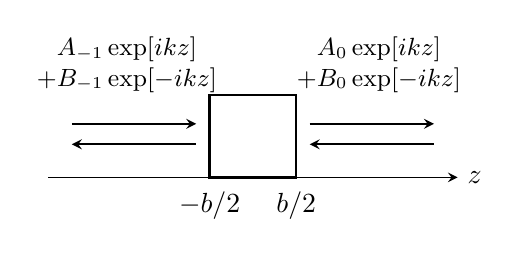
\begin{tikzpicture}[>=stealth, thick, scale=1.0]
  \draw[->, line width=0.55pt] (-2.6, 0) -- (2.6, 0) node[right] {$z$};
  \draw[line width=0.85pt] (-0.55, 0) rectangle (0.55, 1.05);
  \node[below] at (-0.55, -0.05) {$-b/2$};
  \node[below] at (0.55, -0.05) {$b/2$};

  % Left region arrows
  \draw[->, line width=0.6pt] (-2.3, 0.68) -- (-0.72, 0.68);
  \draw[<-, line width=0.6pt] (-2.3, 0.42) -- (-0.72, 0.42);
  % Right region arrows
  \draw[->, line width=0.6pt] (0.72, 0.68) -- (2.3, 0.68);
  \draw[<-, line width=0.6pt] (0.72, 0.42) -- (2.3, 0.42);

  \node[above, align=center, font=\small] at (-1.6, 0.95) {$A_{-1}\exp[ikz]$ \\ $+ B_{-1}\exp[-ikz]$};
  \node[above, align=center, font=\small] at (1.6, 0.95) {$A_0\exp[ikz]$ \\ $+ B_0\exp[-ikz]$};
\end{tikzpicture}
\end{document}
